\documentclass[a4paper,12pt]{article} 
% 使用ctex包支持中文
\usepackage{ctex}
\usepackage{amsmath}
% 开始文档
\usepackage{color}
\usepackage{graphicx}
\begin{document}

% 创建标题页的内容
\title {八省联考导数压轴}
\author{潘世维}
\date{Friday, 20 October 2021}
\maketitle

已知函数 $ f(x)=e^{x}-\sin x-\cos x, g(x)=e^{x}+\sin x+\cos x$


(1) 证明: 当 $ x>-\frac{5 \pi}{4}  时,  f(x) \geq 0 $



(2) 若 $ g(x) \geq 2+a x $, 求  a 
\begin{flushleft}
~\\
\textcolor{red}{证法1:}\\
证明$e^x \ge \sin x + \cos x = \sqrt 2 \sin \left( x + \frac{\pi }{4} \right) $
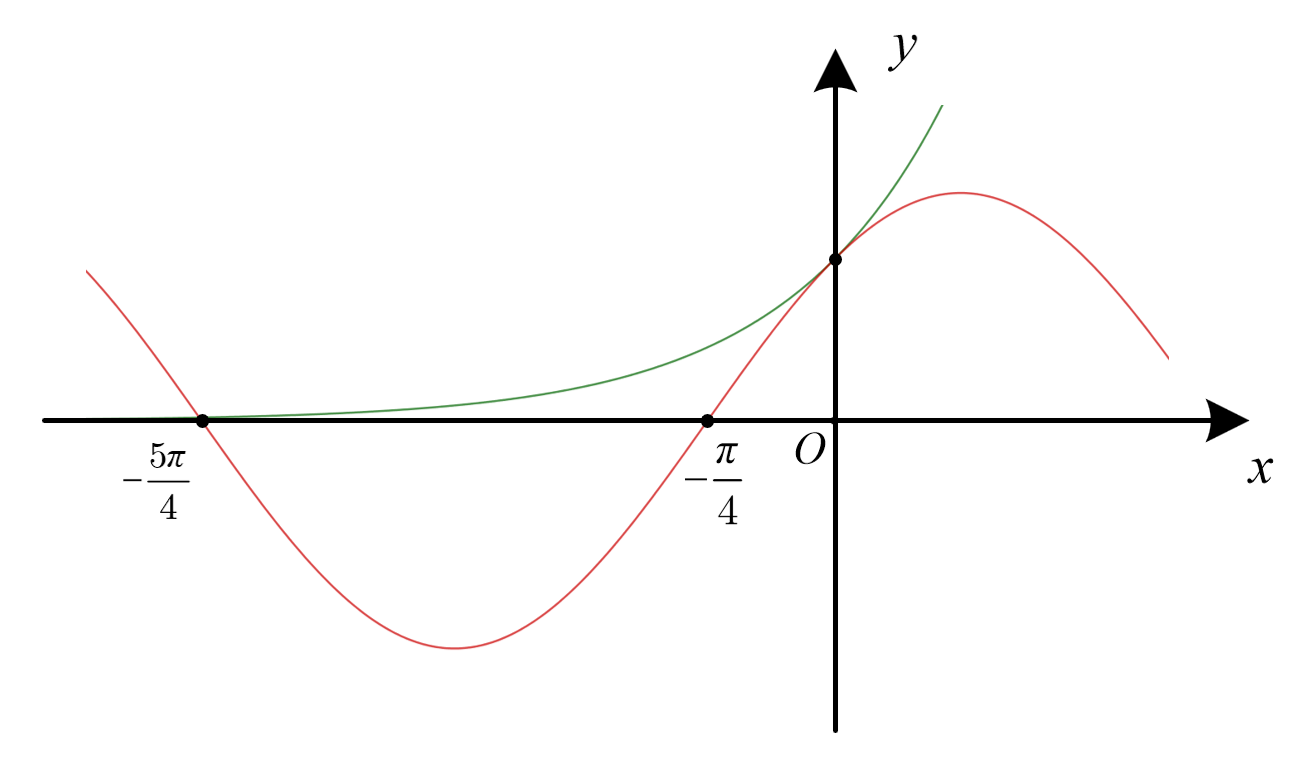
\includegraphics[scale=0.2]{D:/OneDrive/document/8 provinces/pic/pic1.png}\\
①$x \in \left( { - \frac{{5\pi }}{4}, - \frac{\pi }{4}} \right],{e^x} > 0,\sqrt 2 \sin \left( {x + \frac{\pi }{4}} \right) \le 0 \Rightarrow f(x) > 0$

②$x \in \left( { - \frac{\pi }{4},\frac{\pi }{4}} \right),f'(x) = {e^x} - \cos x + \sin x,f''(x) = {e^x} + \sqrt 2 \sin \left( {x + \frac{\pi }{4}} \right) > 0$

$  f'(0) = 0 \Rightarrow f(x) \ge f(0) = 0$

③$\left. {x \in \left[ {\frac{\pi }{4}, + \infty } \right.} \right)\because {e^x} \ge {e^{\frac{\pi }{4}}},\sin x + \cos x \le \sqrt 2 ,{\left( {{e^{\frac{\pi }{2}}}} \right)^{\frac{1}{2}}} > {2^{\frac{1}{2}}} \Rightarrow f(x) > 0$

\end{flushleft}
\end{document}  